\documentclass[11pt,a4paper]{article}

% Typeface: XeLaTeX with Latin Modern Roman (fontspec default)
\usepackage{fontspec}
\usepackage{polyglossia}
\setdefaultlanguage[variant=british]{english}

% Page: the measures of the note template (A4, 11 pt, 4.5 cm side margins, header and page count)
\usepackage[a4paper,left=4.5cm,right=4.5cm,top=4.5cm,bottom=4.1cm,headheight=14pt,headsep=0.55cm,
  footskip=0.55cm]{geometry}
\linespread{0.946}
\usepackage{fancyhdr}
\usepackage{lastpage}
\pagestyle{fancy}
\fancyhf{}
\fancyhead[L]{\small\textbf{PROJECT NOTE} $|$ CLT-Zoo-exercise}
\fancyhead[R]{\small\textbf{Compiled on:} \notedate}
\fancyfoot[C]{\small\thepage\,/\,\pageref{LastPage}}
\renewcommand{\headrulewidth}{0.4pt}

\usepackage{microtype}
\usepackage{amsmath,amssymb}
\usepackage{booktabs,array,tabularx}
\usepackage{graphicx}
\usepackage{enumitem}
\setlist{noitemsep, topsep=3pt, leftmargin=*}
\usepackage{xcolor}
\definecolor{secblue}{HTML}{1F3A5F}
\definecolor{boxback}{HTML}{EEF2F6}
\definecolor{mark}{HTML}{9B2226}
\definecolor{hl}{HTML}{FFF36B}
\usepackage{titlesec}
\titleformat{\section}{\color{secblue}\bfseries\normalsize}{\thesection.}{0.4em}{}
\titlespacing*{\section}{0pt}{10pt}{4pt}
\usepackage[font=small,labelfont=bf,labelsep=period,skip=4pt]{caption}
\usepackage[bottom]{footmisc}
\usepackage{placeins}
\setlength{\parindent}{0pt}
\setlength{\parskip}{5pt}
\setlength{\textfloatsep}{10pt}
\emergencystretch=3em

\newcommand{\notedate}{\number\day\space\ifcase\month\or January\or February\or March\or April\or May\or June\or
  July\or August\or September\or October\or November\or December\fi\space\number\year}

\newcommand{\CdfErrPareto}{0.022}
\newcommand{\CdfErrUniform}{0.0093}
\newcommand{\CdfErrExponential}{0.0027}
\newcommand{\UniformWindowFrom}{$-$7.2}
\newcommand{\UniformWindowTo}{7.2}
\newcommand{\UniformSilent}{92}
\newcommand{\UniformPositions}{302}
\newcommand{\BinomFails}{30}
\newcommand{\BinomPositions}{299}
\newcommand{\NegbinFails}{46}
\newcommand{\NegbinPositions}{179}
\newcommand{\AllPositions}{2,844}
\newcommand{\VtwoErrors}{0}
\newcommand{\MaxCdfErrOthers}{0.0027}
\newcommand{\PosT}{80}
\newcommand{\NoMeanT}{1}
\newcommand{\NoVarT}{2}
\newcommand{\PosPareto}{93}
\newcommand{\NoMeanPareto}{3}
\newcommand{\NoVarPareto}{13}
\newcommand{\PosF}{160}
\newcommand{\NoMeanF}{2}
\newcommand{\NoVarF}{4}
\newcommand{\SlopeA}{$-$0.491}
\newcommand{\TheoryA}{$-$0.500}
\newcommand{\SlopeFirstA}{$-$0.435}
\newcommand{\SlopeLastA}{$-$0.495}
\newcommand{\MedianA}{0.00303}
\newcommand{\SlopeB}{$-$0.332}
\newcommand{\TheoryB}{$-$0.333}
\newcommand{\SlopeFirstB}{$-$0.294}
\newcommand{\SlopeLastB}{$-$0.346}
\newcommand{\MedianB}{0.0497}
\newcommand{\SlopeC}{0.272}
\newcommand{\TheoryC}{0.250}
\newcommand{\SlopeFirstC}{0.336}
\newcommand{\SlopeLastC}{0.267}
\newcommand{\MedianC}{102}
\newcommand{\CltPredA}{0.00318}
\newcommand{\PathFinalC}{150}
\newcommand{\Noise}{0.0061}
\newcommand{\DParetoSim}{0.114}
\newcommand{\DFSim}{0.039}
\newcommand{\DLognormalSim}{0.030}
\newcommand{\DBernoulli}{0.072}
\newcommand{\DExpExact}{0.024}
\newcommand{\DExpSim}{0.027}
\newcommand{\CdBer}{0.3989}
\newcommand{\CeBer}{0.0000}
\newcommand{\NdBer}{1,592}
\newcommand{\NeBer}{4}
\newcommand{\NEBer}{0.0272}
\newcommand{\CdBin}{0.0892}
\newcommand{\CeBin}{0.0000}
\newcommand{\NdBin}{80}
\newcommand{\NeBin}{1}
\newcommand{\NEBin}{0.0014}
\newcommand{\CdPoi}{0.1330}
\newcommand{\CePoi}{0.0332}
\newcommand{\NdPoi}{177}
\newcommand{\NePoi}{11}
\newcommand{\NEPoi}{3.3245}
\newcommand{\CdGeo}{0.2066}
\newcommand{\CeGeo}{0.1351}
\newcommand{\NdGeo}{427}
\newcommand{\NeGeo}{183}
\newcommand{\NEGeo}{13.5101}
\newcommand{\CdNb}{0.1075}
\newcommand{\CeNb}{0.0614}
\newcommand{\NdNb}{116}
\newcommand{\NeNb}{38}
\newcommand{\NENb}{6.1421}


\begin{document}


\vspace*{14pt}
\begin{tabular}{@{}p{2.35cm}@{}p{\dimexpr\textwidth-2.35cm}@{}}
\textbf{TITLE:} & \textbf{\large The CLT Zoo: sixteen distributions, where the Law of Large Numbers and the Central Limit Theorem hold, and how
far the normal approximation is for discrete sums}\\[3pt]
\textbf{SUBJECT:} & Aim, method and results of the analyses in version 2 of the \texttt{CLT-Zoo-exercise} repository\\[3pt]
\textbf{AUTHOR:} & Muhammed İkbal Yılmaz (myucanlar@gmail.com)
\end{tabular}

\vspace{8pt}
\vspace{12pt}

\section{Aim and scope}

Version 1 of this project is a notebook with sixteen distributions (eleven continuous, five discrete), each with its parameter
sliders and a preset. Its introduction and README describe a study of the Law of Large Numbers (LLN) and the Central Limit Theorem
(CLT): a running mean, the sampling distribution of the mean for a sample size $N$ and $M$ Monte Carlo replications, the
standardized mean against $\mathcal N(0,1)$, and normal curves that are switched off when the mean or the variance is infinite. The
code does not contain any of these. It is a distribution explorer: for one distribution it draws the density or probability
function, a sample, and a distribution function obtained by integrating the density numerically. Version 2 keeps the zoo as it is
(names, parameters, slider ranges, presets, samplers, seed 42), corrects the explorer, adds the LLN and CLT views the README
described, and asks three questions:

\begin{enumerate}
  \item \textbf{Is the zoo correct, and what did the explorer of version 1 compute?} Analysis 1.
  \item \textbf{Where on the sliders does the LLN hold, and how fast?} The Pareto slider alone covers the three regimes. Analysis 2.
  \item \textbf{How close is the standardized mean to $\mathcal N(0,1)$ across the zoo, and exactly for the five discrete members?}
  Analysis 3.
\end{enumerate}

\section{The zoo and its moments}

For a distribution with mean $\mu$ and variance $\sigma^2$, the skewness is $\gamma = E(X-\mu)^3/\sigma^3$ and the excess kurtosis
$\kappa = E(X-\mu)^4/\sigma^4 - 3$. The \emph{moment order} $r^\ast$ is the number with $E|X|^r < \infty$ exactly for $r < r^\ast$:
$r^\ast = \infty$ for every member of the zoo except Student-t ($r^\ast = \nu$), Pareto ($r^\ast = \alpha$) and F
($r^\ast = d_2/2$). The mean exists if $r^\ast > 1$, the variance if $r^\ast > 2$. The samplers are those of version 1
(\texttt{numpy.random.Generator}); Table~\ref{tab:zoo} gives the parametrization they use.

\begin{table}[h]
\centering\scriptsize\setlength{\tabcolsep}{3pt}
\caption{The sixteen distributions of version 1: parameters (names of version 1), mean and variance. Geometric counts trials up to
the first success ($1, 2, \dots$); Negative Binomial counts failures before the $r$-th success ($0, 1, \dots$); Pareto has
$P(X > x) = (x_m/x)^{\alpha}$ for $x \ge x_m$.}\label{tab:zoo}
\begin{tabular}{lll}
\toprule
Distribution & Mean & Variance \\
\midrule
Normal$(\mu,\sigma)$ & $\mu$ & $\sigma^2$ \\
Uniform$(a,b)$ & $(a+b)/2$ & $(b-a)^2/12$ \\
Exponential(scale $s$) & $s$ & $s^2$ \\
Gamma$(k,\theta)$ & $k\theta$ & $k\theta^2$ \\
Beta$(\alpha,\beta)$ & $\dfrac{\alpha}{\alpha+\beta}$ & $\dfrac{\alpha\beta}{(\alpha+\beta)^2(\alpha+\beta+1)}$ \\
Lognormal$(m,s)$ & $e^{m+s^2/2}$ & $(e^{s^2}-1)e^{2m+s^2}$ \\
Laplace$(\mu,b)$ & $\mu$ & $2b^2$ \\
Student-t$(\nu)$ & $0$ \ ($\nu>1$) & $\nu/(\nu-2)$ \ ($\nu>2$) \\
Pareto$(x_m,\alpha)$ & $\alpha x_m/(\alpha-1)$ \ ($\alpha>1$) & $x_m^2\alpha/[(\alpha-1)^2(\alpha-2)]$ \ ($\alpha>2$) \\
Chi-square$(k)$ & $k$ & $2k$ \\
F$(d_1,d_2)$ & $d_2/(d_2-2)$ \ ($d_2>2$) & $\dfrac{2d_2^2(d_1+d_2-2)}{d_1(d_2-2)^2(d_2-4)}$ \ ($d_2>4$) \\
Bernoulli$(p)$, Binomial$(n,p)$ & $p$, \ $np$ & $p(1-p)$, \ $np(1-p)$ \\
Poisson$(\lambda)$ & $\lambda$ & $\lambda$ \\
Geometric$(p)$, NegBinomial$(r,p)$ & $1/p$, \ $r(1-p)/p$ & $(1-p)/p^2$, \ $r(1-p)/p^2$ \\
\bottomrule
\end{tabular}
\end{table}

\section{Theory and methods}

\textbf{LLN and CLT.} Let $X_1, X_2, \dots$ be independent copies of $X$, $S_n = X_1 + \dots + X_n$ and $\bar X_n = S_n/n$. If
$E|X| < \infty$, then $\bar X_n \to \mu$ (Kolmogorov, 1933). If also $\sigma^2 < \infty$, then
$Z_n = \sqrt{n}\,(\bar X_n - \mu)/\sigma \xrightarrow{d} \mathcal N(0,1)$ (Lindeberg, 1922; Lévy, 1937), so that
$|\bar X_n - \mu|$ is of order $n^{-1/2}$.

\textbf{Without a finite variance} (Gnedenko and Kolmogorov, 1954; Feller, 1971). For Pareto$(1,\alpha)$ the tail
$P(X > x) = x^{-\alpha}$ puts $X$ in the domain of attraction of a stable law of index $\alpha$ when $\alpha < 2$. For
$1 < \alpha < 2$, $n^{1-1/\alpha}(\bar X_n - \mu)$ converges to a stable law, so $|\bar X_n - \mu|$ is of order
$n^{1/\alpha - 1}$, slower than $n^{-1/2}$. For $\alpha < 1$ the mean is infinite and $S_n/n^{1/\alpha} = n^{1-1/\alpha}\bar X_n$
converges to a positive stable law, so $\bar X_n$ grows like $n^{1/\alpha - 1}$. Analysis 2 measures these exponents:
$-1/2$ ($\alpha = 2.5$), $-1/3$ ($\alpha = 1.5$) and $+1/4$ ($\alpha = 0.8$).

\textbf{Exact law of the sum.} For nine members $S_N$ has a closed form, which makes the distribution of $Z_N$ exact:
\begin{equation}
\begin{aligned}
&\text{Normal}: \ \mathcal N(N\mu, N\sigma^2); \quad \text{Exponential}(s): \ \text{Gamma}(N, s); \\
&\text{Gamma}(k,\theta): \ \text{Gamma}(Nk, \theta); \quad \chi^2_k: \ \chi^2_{Nk}; \\
&\text{Bernoulli}(p): \ \text{Bin}(N, p); \quad \text{Bin}(n,p): \ \text{Bin}(Nn, p); \\
&\text{Poisson}(\lambda): \ \text{Poisson}(N\lambda); \\
&\text{Geometric}(p): \ N + \text{NegBin}(N, p); \quad \text{NegBin}(r,p): \ \text{NegBin}(Nr, p).
\end{aligned}\label{eq:sums}
\end{equation}

\textbf{Distance to the normal law.} With $F_N(x) = P(Z_N \le x)$ and $\Phi$ the standard normal distribution function, the
Kolmogorov distance is $D_N = \sup_x |F_N(x) - \Phi(x)|$. For an integer-valued $S_N$, $F_N$ is constant between the points
$z_k = (k - N\mu)/(\sigma\sqrt N)$, so the supremum is attained at some $z_k$, either at the point or just before it:
\begin{equation}
\begin{split}
D_N = \max_k \max\bigl(&|P(S_N \le k) - \Phi(z_k)|,\\
&|P(S_N \le k-1) - \Phi(z_k)|\bigr),
\end{split}
\label{eq:dlattice}
\end{equation}
over every $k$ that carries probability (all but $10^{-15}$ in each tail). For a continuous $S_N$, the supremum is located on a grid
of step 0.001 on $[-10, 10]$ and refined by bounded scalar optimization. The \emph{continuity correction} approximates
$P(S_N \le k)$ by $\Phi$ at the midpoint between two lattice values; its error is
\begin{equation}
E_N = \max_k \Bigl|P(S_N \le k) - \Phi\Bigl(\frac{k + \tfrac12 - N\mu}{\sigma\sqrt N}\Bigr)\Bigr|. \label{eq:corrected}
\end{equation}

\textbf{Why the correction helps, and by how much.} For an integer-valued $X$ whose values have greatest common step 1 (true for all
five discrete presets), the lattice Edgeworth expansion (Esseen, 1945; Gnedenko and Kolmogorov, 1954) is
\begin{equation}
\begin{split}
F_N(x) - \Phi(x) &= \Bigl[-\frac{\gamma}{6}(x^2 - 1) + \frac{1}{\sigma}\, Q\bigl(N\mu + \sigma\sqrt N x\bigr)\Bigr]\frac{\varphi(x)}{\sqrt N}
+ o\bigl(N^{-1/2}\bigr),\\
Q(t) &= \lfloor t \rfloor - t + \tfrac12 ,
\end{split}
\label{eq:edgeworth}
\end{equation}
where $\varphi$ is the standard normal density. The first term is the skewness correction of continuous distributions; the second,
a saw-tooth with values in $[-\tfrac12, \tfrac12]$, is the lattice term: it takes both extreme values next to every jump of $F_N$
and is zero at the midpoints, which is why the continuity correction removes it. Both terms are largest in absolute value at
$x = 0$, which gives the leading constants
\begin{equation}
\begin{split}
\sqrt N\, D_N &\to c_D = \varphi(0)\Bigl(\frac{1}{2\sigma} + \frac{|\gamma|}{6}\Bigr), \qquad
\sqrt N\, E_N \to c_E = \varphi(0)\,\frac{|\gamma|}{6},\\
\varphi(0) &= 1/\sqrt{2\pi}.
\end{split}
\label{eq:constants}
\end{equation}
For symmetric members ($\gamma = 0$) $c_E = 0$ and $E_N$ is of order $1/N$. Analysis 3 checks \eqref{eq:constants} against the
exact distances.

\textbf{Simulation.} Sample means are computed from $M$ rows of $N$ draws. The distance of $M$ simulated values of $Z_N$ to
$\Phi$ contains noise; for $M = 20{,}000$ its mean, when $Z_N$ is exactly $\mathcal N(0,1)$, is \Noise{} (exact distribution of the
Kolmogorov statistic).

\textbf{From the equations to the code.} Each step is a function in \texttt{cltzoo/} and is checked in \texttt{tests/run\_tests.py}
against an independent computation (the code of version 1 read from the legacy notebook, numerical integration of the densities,
$N$-fold convolution, goodness-of-fit tests of the samplers, brute-force search on a fine grid):

\begin{center}\footnotesize
\begin{tabularx}{\textwidth}{@{}>{\raggedright\arraybackslash}p{2.3cm}>{\raggedright\arraybackslash}p{2.0cm}>{\raggedright\arraybackslash}X@{}}
\toprule
Step & Equations & Code \\
\midrule
Zoo, moments, $r^\ast$ & Table~\ref{tab:zoo} & \texttt{ZOO[name].sample / .frozen / .moments / .moment\_order} \\
Law of $S_N$ & \eqref{eq:sums} & \texttt{ZOO[name].sum\_law(N)} \\
$D_N$, $E_N$ & \eqref{eq:dlattice}, \eqref{eq:corrected} & \texttt{kolmogorov\_distance}, \texttt{corrected\_error} \\
Lattice constants & \eqref{eq:constants} & \texttt{lattice\_constants} \\
Running mean, sample means & --- & \texttt{running\_mean}, \texttt{running\_mean\_quantiles}, \texttt{sample\_means} \\
Notebook views & --- & \texttt{panels.explorer\_figure}, \texttt{panels.clt\_figure}, \texttt{widgets} \\
\bottomrule
\end{tabularx}
\end{center}

\section{Analysis 1: The zoo and the explorer of version 1 (Figure~\ref{fig:zoo})}

\textbf{Why.} Every later result rests on the distributions being what they claim to be, and on knowing where their moments exist.

\textbf{Method.} The samplers, densities and moments of version 2 are compared with version 1 and with independent computations
(unit tests). The code of version 1 is then run on its own presets: its distribution function, the integral of the density over
the plotting window rescaled to end at 1, is compared with the exact one. Its density or probability function is also evaluated at
every slider position of every parameter, the other parameters at their presets.

\textbf{How to read the figure.} Each panel: a sample of seed 42 (bars) and the exact density or probability function (line or
dots), at the preset of version 1.

\begin{figure}[h]
\centering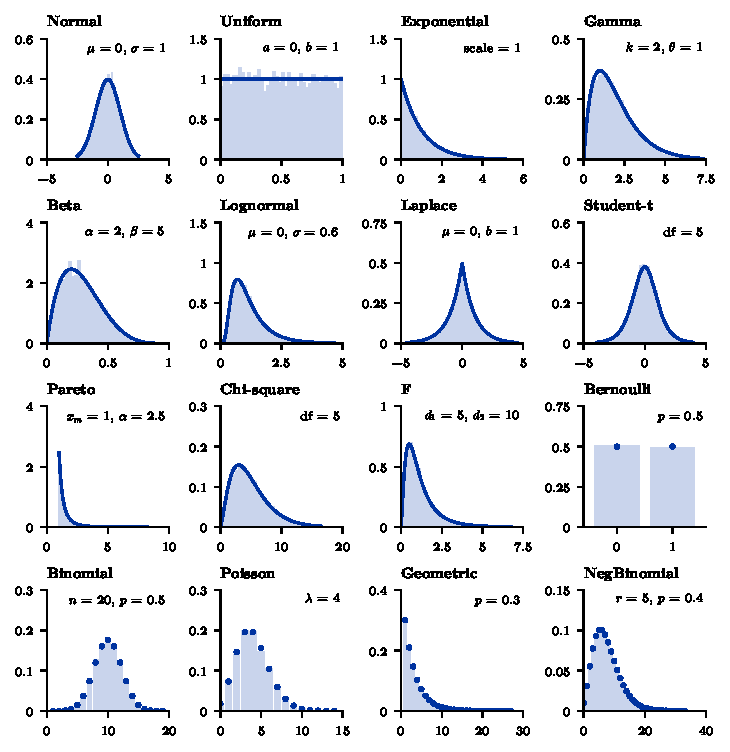
\includegraphics[width=\textwidth]{../figures/fig1_zoo.pdf}
\caption{The zoo at the presets of version 1: exact density or probability function and a sample of seed 42 (the preset sample
size of version 1, or 6,000 draws where its preset showed no sample).}\label{fig:zoo}
\end{figure}

\textbf{Finding.} The sixteen samplers of version 1 are correct: version 2 reproduces their draws exactly, and each agrees with its
exact law (Kolmogorov--Smirnov or chi-square test, 200,000 draws). Its densities and probability functions are exact. Its
distribution function is not: the largest error is \CdfErrPareto{} for Pareto, where the density jumps at $x_m$, and
\CdfErrUniform{} for Uniform, whose window ran from \UniformWindowFrom{} to \UniformWindowTo{} for a support of $[0, 1]$; for the
other presets it is at most \MaxCdfErrOthers. The probability functions of Binomial and Negative Binomial stopped with an
\texttt{OverflowError} at \BinomFails{} of \BinomPositions{} and \NegbinFails{} of \NegbinPositions{} slider positions
($n \ge 171$; $r \ge 45$ or $p \le 0.10$): the binomial coefficients were computed from \texttt{math.gamma}, which overflows
for arguments above 171.6. The exact functions of version 2 are finite at all \AllPositions{} valid slider positions (\VtwoErrors{}
failures). At \UniformSilent{}
of \UniformPositions{} positions of the Uniform sliders $b \le a$, and version 1 replaced $b$ silently by $a + 10^{-6}$. The mean
does not exist at \NoMeanPareto{} of the \PosPareto{} Pareto positions, \NoMeanT{} of the \PosT{} Student-t positions and \NoMeanF{}
of the \PosF{} positions of $d_2$ for F; the variance at \NoVarPareto, \NoVarT{} and \NoVarF{} of them.

\textbf{Interpretation.} The zoo itself needed no change. Version 2 uses exact distribution functions from \texttt{scipy.stats},
reports an impossible Uniform range instead of altering it, and knows where the mean and the variance exist, which the LLN and CLT
views need.

\section{Analysis 2: The LLN on the Pareto slider (Figure~\ref{fig:lln})}

\textbf{Why.} The README of version 1 promised a running mean and normal curves that switch off when the mean or variance is
infinite. Its Pareto slider ($\alpha$ from 0.8 to 10) contains all three regimes of Section 3, so the theory can be checked where
the notebook lets the user go.

\textbf{Method.} Pareto$(1,\alpha)$ for $\alpha = 2.5$ (the preset), 1.5 and 0.8 (the smallest slider value). One running mean of
$10^5$ draws each (seed 42); then, over 4,000 independent paths, the median of $|\bar X_n - \mu|$ ($\alpha = 2.5, 1.5$) or of
$\bar X_n$ ($\alpha = 0.8$) at 21 values of $n$ from 10 to $10^5$. The slope of its logarithm against $\log n$ is fitted for $n$
from $10^3$ to $10^5$ and in each decade of $n$.

\textbf{How to read the figure.} (a) Dotted lines: $\mu$. (b) Log--log scale: a straight line of slope $s$ means a power $n^{s}$;
the band holds the middle half of the paths; dotted lines have the theoretical slope.

\begin{figure}[h]
\centering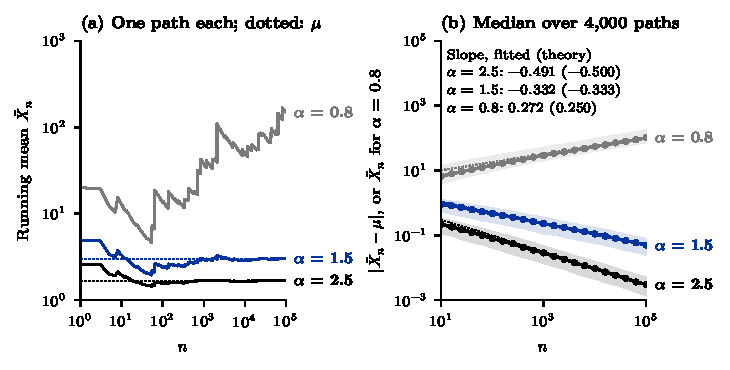
\includegraphics[width=\textwidth]{../figures/fig2_lln.pdf}
\caption{The LLN for Pareto$(1, \alpha)$: (a) one running mean for each $\alpha$; (b) median distance to $\mu$ (or median running
mean when $\mu = \infty$) over 4,000 paths, with quartiles.}\label{fig:lln}
\end{figure}

\textbf{Finding.} The fitted slopes are \SlopeA{} ($\alpha = 2.5$, theory \TheoryA), \SlopeB{} ($\alpha = 1.5$, theory \TheoryB) and
\SlopeC{} ($\alpha = 0.8$, theory \TheoryC). The local slopes move toward the theoretical values as $n$ grows: from \SlopeFirstA{}
($n$ from 10 to 100) to \SlopeLastA{} ($10^4$ to $10^5$) for $\alpha = 2.5$, and from \SlopeFirstC{} to \SlopeLastC{} for
$\alpha = 0.8$; for $\alpha = 1.5$ they lie between \SlopeFirstB{} and \SlopeLastB. At $n = 10^5$ the median of $|\bar X_n - \mu|$
for $\alpha = 2.5$ is \MedianA, against $0.6745\,\sigma/\sqrt n = \CltPredA$ from the CLT. For $\alpha = 0.8$ the single path ends
at \PathFinalC{} and the median running mean is \MedianC.

\textbf{Interpretation.} With a finite variance the error falls like $n^{-1/2}$; with $1 < \alpha \le 2$ the mean is still
estimated consistently, but at the slower rate $n^{1/\alpha - 1}$, and no normal curve describes the error; with $\alpha \le 1$
there is nothing to converge to. Exponents measured on finite paths approach their limits only slowly, as the local slopes show.
This is the behaviour the notebook now shows: in the LLN and CLT view
the line for $\mu$ is drawn only when $\mu$ is finite, and the normal curves only when $\sigma^2$ is finite.

\FloatBarrier
\section{Analysis 3: The CLT across the zoo, and exactly for discrete sums (Table~\ref{tab:lattice}, Figures~\ref{fig:clt}, \ref{fig:lattice})}

\textbf{Why.} The README of version 1 promised the standardized mean against $\mathcal N(0,1)$ for every member. For the five
discrete members the distribution function of $Z_N$ jumps, which sets a floor of order $1/\sqrt N$ on its distance to any continuous
law; by \eqref{eq:sums} it can be computed exactly.

\textbf{Method.} (A) Every preset, $N = 30$: 20,000 sample means (seed 42) and the distance of their $Z_{30}$ to $\Phi$; for the
nine members of \eqref{eq:sums} also the exact $D_{30}$. (B) The five discrete presets: exact $D_N$ \eqref{eq:dlattice} and $E_N$
\eqref{eq:corrected} for $N$ from 1 to $10^4$, compared with \eqref{eq:constants}; and the smallest $N$ with $D_N < 0.01$ and with
$E_N < 0.01$, searched up to $N = 3{,}000$.

\textbf{How to read the figures.} Figure~\ref{fig:clt}: histograms of $Z_{30}$ with the $\mathcal N(0,1)$ density; for discrete
members each bar covers whole lattice values. Figure~\ref{fig:lattice}: log--log scale; dotted lines are $c/\sqrt N$ with $c$ from
\eqref{eq:constants}; the red dotted line is 0.01.

\begin{figure}[h]
\centering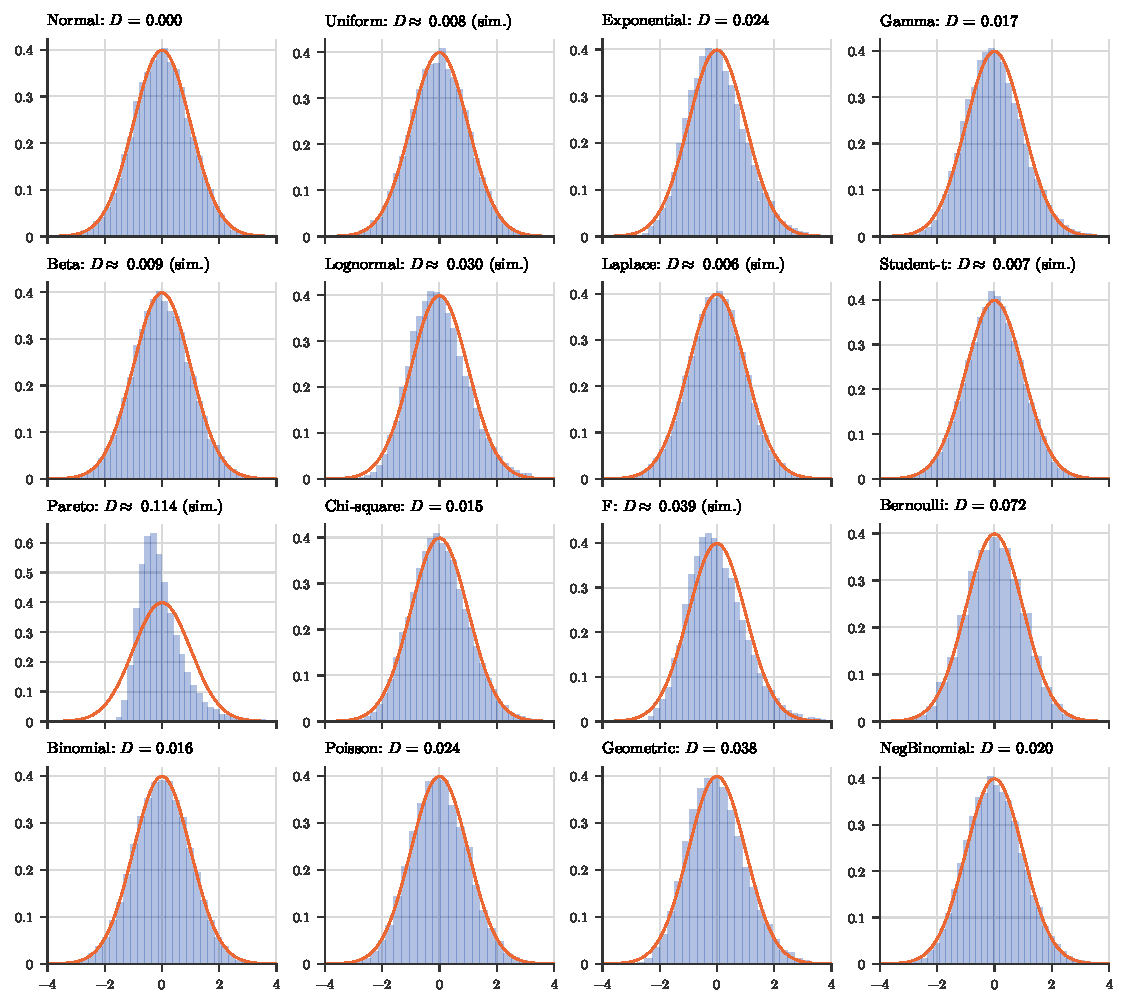
\includegraphics[width=\textwidth]{../figures/fig3_clt_n30.pdf}
\caption{Standardized mean $Z_{30}$ at every preset (20,000 sample means, seed 42) with the $\mathcal N(0,1)$ density, and the
distance $D$ to $\mathcal N(0,1)$: exact where the law of $S_{30}$ is known, otherwise from the simulation.}\label{fig:clt}
\end{figure}

\begin{table}[h]
\centering\footnotesize
\caption{(Top) $N = 30$: skewness $\gamma/\sqrt{30}$ of $Z_{30}$, exact $D_{30}$ where available, and $D$ from 20,000 simulated
values (noise level \Noise). (Bottom) Discrete presets: $\sigma$, $\gamma$, the constants \eqref{eq:constants} with $\sqrt N D_N$
and $\sqrt N E_N$ at $N = 10^4$, and the smallest $N$ with $D_N < 0.01$ and with $E_N < 0.01$ (both stay below 0.01 for every
larger $N$ up to 3,000).}\label{tab:lattice}
\begin{tabular}[t]{lrrr}
\toprule
 & $\gamma/\sqrt{30}$ & exact & sim. \\
\midrule
Normal & 0.000 & 0.000 & 0.007 \\
Uniform & 0.000 &  & 0.008 \\
Exponential & 0.365 & 0.024 & 0.027 \\
Gamma & 0.258 & 0.017 & 0.018 \\
Beta & 0.109 &  & 0.009 \\
Lognormal & 0.413 &  & 0.030 \\
Laplace & 0.000 &  & 0.006 \\
Student-t & 0.000 &  & 0.007 \\
Pareto & -- &  & 0.114 \\
Chi-square & 0.231 & 0.015 & 0.016 \\
F & 0.706 &  & 0.039 \\
Bernoulli & 0.000 & 0.072 & 0.074 \\
Binomial & 0.000 & 0.016 & 0.020 \\
Poisson & 0.091 & 0.024 & 0.030 \\
Geometric & 0.371 & 0.038 & 0.039 \\
NegBinomial & 0.169 & 0.020 & 0.019 \\
\bottomrule

\end{tabular}

\medskip
\setlength{\tabcolsep}{3.5pt}
\begin{tabular}[t]{lrrrrrrrr}
\toprule
 & $\sigma$ & $\gamma$ & $c_D$ & $\sqrt N D_N$ & $c_E$ & $\sqrt N E_N$ & $N_D$ & $N_E$ \\
\midrule
Bernoulli & 0.500 & 0.000 & 0.3989 & 0.3989 & 0.0000 & 0.0003 & 1,592 & 4 \\
Binomial & 2.236 & 0.000 & 0.0892 & 0.0892 & 0.0000 & 0.0000 & 80 & 1 \\
Poisson & 2.000 & 0.500 & 0.1330 & 0.1330 & 0.0332 & 0.0332 & 177 & 11 \\
Geometric & 2.789 & 2.032 & 0.2066 & 0.2066 & 0.1351 & 0.1351 & 427 & 183 \\
NegBinomial & 4.330 & 0.924 & 0.1075 & 0.1075 & 0.0614 & 0.0614 & 116 & 38 \\
\bottomrule

\end{tabular}
\end{table}

\begin{figure}[h]
\centering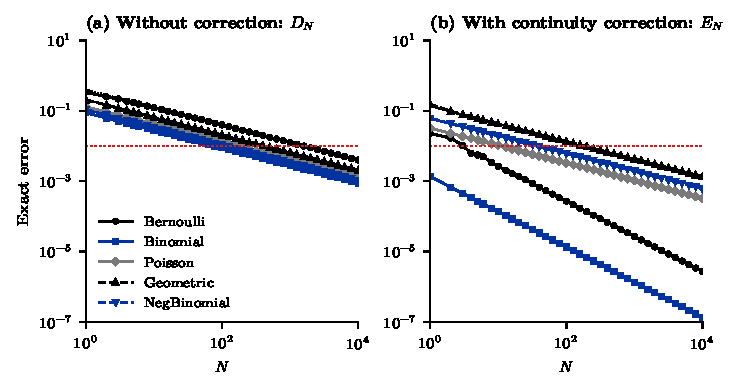
\includegraphics[width=\textwidth]{../figures/fig4_lattice.pdf}
\caption{Discrete presets: exact distance of $Z_N$ to $\mathcal N(0,1)$, (a) without and (b) with the continuity correction.
Dotted: $c/\sqrt N$ from the lattice Edgeworth expansion.}\label{fig:lattice}
\end{figure}

\textbf{Finding.} At $N = 30$ the largest distances belong to the members with heavy or very skewed tails: Pareto
(\DParetoSim, no finite third moment), F (\DFSim) and Lognormal (\DLognormalSim), and to Bernoulli (\DBernoulli), whose standardized
mean takes only 31 values. Where the exact value is known the simulated distance agrees with it up to the noise level (Exponential:
\DExpExact{} exact, \DExpSim{} simulated). For the five discrete presets $\sqrt N D_N$ and $\sqrt N E_N$ at $N = 10^4$ equal the
constants of \eqref{eq:constants} to four decimals (Table~\ref{tab:lattice}). Without the correction, $D_N < 0.01$ requires
$N = \NdBer$ for Bernoulli and between \NdBin{} and \NdGeo{} for the others; with it, $N = \NeBer$, \NeBin, \NePoi, \NeNb{} and
\NeGeo{} suffice (Bernoulli, Binomial, Poisson, Negative Binomial, Geometric). For the symmetric members $N E_N$ settles at
\NEBer{} (Bernoulli) and \NEBin{} (Binomial), so $E_N$ falls like $1/N$.

\textbf{Interpretation.} For a discrete population the error of the normal approximation has two parts of the same order
$1/\sqrt N$: the jumps of the lattice and the skewness. The continuity correction removes the first exactly and leaves the second,
so it is most useful for symmetric distributions (Bernoulli with $p = 0.5$: $N = \NeBer$ instead of \NdBer) and least for skewed
ones (Geometric: \NeGeo{} instead of \NdGeo). A distance of 0.01 is reached at very different $N$ across the zoo, so a single rule
such as $N \ge 30$ does not describe it.

\FloatBarrier
\section{Conclusions and limitations}

\begin{itemize}
  \item The zoo of version 1 is correct: samplers and densities are reproduced exactly. Its distribution functions were numerical
  (error up to \CdfErrPareto), Binomial and Negative Binomial failed at \BinomFails{} and \NegbinFails{} slider positions, and an
  impossible Uniform range was changed silently. Version 2 fixes all three and adds the LLN and CLT views that its README described.
  \item LLN: on the Pareto slider the error of the mean falls like $n^{-1/2}$, like $n^{1/\alpha-1}$ with infinite variance, and the
  running mean diverges for $\alpha \le 1$; the measured exponents agree with theory to within 0.03 and approach it as $n$ grows.
  \item CLT for discrete sums: the exact distances follow the lattice Edgeworth constants; the continuity correction removes the
  lattice term and leaves the skewness term, which is why it helps symmetric distributions most.
  \item Limitations: one parameter value per member except Pareto; the distances of the six continuous members without a closed-form
  sum are simulated, so below about \Noise{} they cannot be resolved; exact distances for continuous members are the subject of the
  CLT speed race project of the same author.
\end{itemize}

\section*{References}
{\small
\setlength{\parskip}{2pt}
\hangindent=1.27cm\hangafter=1 Esseen, C.-G. (1945). Fourier analysis of distribution functions. A mathematical study of the Laplace--Gaussian law. \textit{Acta
Mathematica}, 77, 1--125.\par
\hangindent=1.27cm\hangafter=1 Feller, W. (1971). \textit{An introduction to probability theory and its applications} (Vol. 2, 2nd ed.). Wiley.\par
\hangindent=1.27cm\hangafter=1 Gnedenko, B. V., \& Kolmogorov, A. N. (1954). \textit{Limit distributions for sums of independent random variables}. Addison-Wesley.\par
\hangindent=1.27cm\hangafter=1 Kolmogorov, A. N. (1933). \textit{Grundbegriffe der Wahrscheinlichkeitsrechnung}. Springer.\par
\hangindent=1.27cm\hangafter=1 Lévy, P. (1937). \textit{Théorie de l'addition des variables aléatoires}. Gauthier-Villars.\par
\hangindent=1.27cm\hangafter=1 Lindeberg, J. W. (1922). Eine neue Herleitung des Exponentialgesetzes in der Wahrscheinlichkeitsrechnung. \textit{Mathematische
Zeitschrift}, 15(1), 211--225.\par
\hangindent=1.27cm\hangafter=1 NumPy and SciPy documentation: \texttt{numpy.random.Generator}, \texttt{scipy.stats}.\par

\smallskip
All numbers are generated from
\texttt{figures/*.csv} by \texttt{make\_paper.py}.
}

\end{document}
